%\documentclass[notes=only]{beamer}
\documentclass{beamer}
\usepackage{pgfpages}
\mode<handout>{%
%	\pgfpagesuselayout{2 on 1}[a4paper] 
	\setbeameroption{show notes}
}
%\documentclass{beamer}
%\usetheme{Montpellier}
\usetheme{Montpellier}
\usepackage{booktabs, colortbl}
\definecolor{lavender}{rgb}{0.9,0.9,0.98}
\usepackage{array}
\newcolumntype{P}[1]{>{\centering\arraybackslash}p{#1}}

\usepackage{xcolor}
\usepackage{listings}
% Setup listing style
\lstdefinestyle{imandra} {
	aboveskip=5pt,
	language=caml,
	keywordstyle=\color{blue},
	commentstyle=\itshape\color{purple},
	stringstyle=\color{brown},
	basicstyle=\ttfamily\footnotesize,
	breakatwhitespace=false,         
	breaklines=true,                 
	captionpos=b,       
	%columns=fixed,             
	keepspaces=true,
	showspaces=false,                
	showstringspaces=false,
	showtabs=false,                  
	tabsize=2,
	inputencoding=utf8,
	extendedchars=true,
	literate={φ}{{$\phi$}}1,
	backgroundcolor=\color{lavender}
}

\lstset{
	style=imandra,
	morekeywords={
		lemma,
		verify,
		theorem, 
		@@measure, 
		@@auto, 
		@@fc, 
		@@blast,
		@@disable,
		@@rw,
		@@unroll
	}
}

\usepackage{svg}

\usepackage[style=authoryear, backend=biber]{biblatex}
\addbibresource{MatrixFormalisation.bib}
%\usepackage{xparse}
%%\usepackage{fullpage}
%%\renewcommand{\baselinestretch}{1.5}
%\renewcommand{\baselinestretch}{1.5}
%\usepackage[hang]{footmisc}
%\setlength\footnotemargin{10pt}
%\usepackage[natbibapa]{apacite}
%\bibliographystyle{apacite}
%\NewDocumentCommand\footcite{ O{} O{} m }{%
%	\footnote{\citet[#1][#2]{#3}.}%
%}

\title{Neural Networks in Imandra: Matrix
Representation as a Verification Choice}
\author{Remi Desmartin\inst{1} \and Ekaterina Komendenskaya\inst{1} \and Grant Passmore\inst{2}}

\institute[VFU] % (optional)
{
	\inst{1}%
	Heriot-Watt University \\ Edinburgh, UK
	\and
	\inst{2}%
	Imandra Inc. \\ Austin, TX, USA
}
\begin{document}
\begin{frame}[plain]
    \maketitle
\end{frame}


\begin{frame}{Neural Networks}

\begin{itemize}
	\item<1-> Ubiquitous
	\item<2-> Safety-critical systems
	\item<3-> Not always reliable\footcite{GoodfellowSS14}
\end{itemize}

\note{NN are more and more often deployed as part of safety-critical systems like self-driving cars, financial algorithms or facial recognition systems. However we know that they have weak points, like adversarial attacks}

\end{frame}

\begin{frame}{Neural Network Verification}

\begin{itemize}
\item<1-> SMT-solvers

\item<1-> Abstract interpretation

\item<2-> Functional programming

\begin{itemize}
	\item<3-> Coq formalisations~\footcite{BS19,de_maria_use_2021}
	\item<3-> Dependent types~\footcite{kokke_neural_2020}
\end{itemize}
\end{itemize}

\end{frame}

\note{As a result, there is an increasing demand for neural network verification tools. Research into NNV tools has been mainly pushed by the SMT-solving community and the Abstract interpretation community.\\
	Recently, claims have been made that functional programming can be valuable in this domain: Coq formalisation of small neuronal archetypes (perceptrons) and importing trained NNs from Python environment (MLCert)
	Work on dependent types: robustness as a dependent type, library in F*.
}

\begin{frame}{Functional Implementations of Neural Networks}
\begin{itemize}
	\item<1-> Generalisation
	\item<2-> Executability
	\item<3-> \textbf{Matrices}
\end{itemize}
\end{frame}

\note{We want our Neural Network implementation in a FPL to be \textbf{executable} (able to perform inference within the same framework where verification is performed) and \textbf{general}, i.e. have reusable components to define different NN models. For this reason, we use matrices for implementing NNs}

\begin{frame}{Imandra}
	\begin{itemize}
		\item Interactive theorem prover
		\item Typed, higher-order lifting of Boyer-Moore waterfall~\footcite{BM79}
		\item Functional programming language - subset of OCaml
		\item Coupled with other proof methods
	\end{itemize}
\end{frame}

\note{Presentation of Imandra\\ Todo: add schema of waterfall; other illustrations?}

\begin{frame}[fragile]{Imandra: Example}

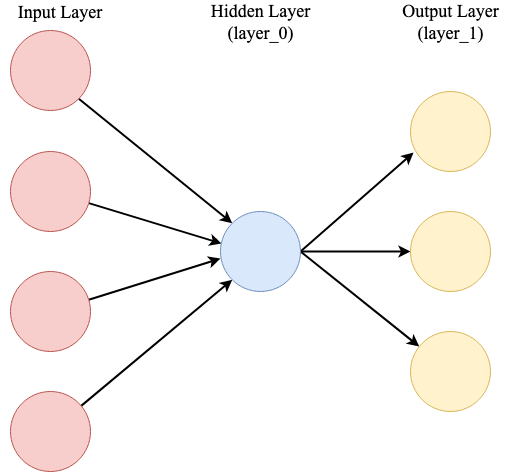
\includegraphics[height=5cm]{figures/mlp_iris.png}

\begin{block}{Goal}
\begin{lstlisting}
	let model input = layer_0 input >>= layer_1 >>= layer_2 >>= layer_4;;
\end{lstlisting}
\end{block}
\end{frame}

\note{the goal is to have a functional defintion of our neural network: function composition where each layeri is a layer represented by a function}

\begin{frame}[fragile]{Neural Network Formalisation in Imandra: an Example}
	\begin{lstlisting}
	type iris_input = {
		sepal_len: real;
		sepal_width: real;
		petal_len: real;
		petal_width: real;
	}
	
	let layer_0 (w0, w1, w2, w3, w4) (f1, f2, f3, f4) =
		relu (w0 +. w1 *. f1 +. w2 *.f2 +. w3 *. f3 +. w4 *. f4)
		
	let weights_0 = (1.0023211, 1.1538234, -0.30127743, 0.9319558, 2.179688)
	
	\end{lstlisting}

\end{frame}
\note{let us take an example to present Imandra's syntax and the necessity for matrices: the Iris dataset, where we classify flowers from 4 measurements into 3 subspecies of Iris \\
	
}

\begin{frame}[fragile]{Neural Network Formalisation in Imandra: an Example}
	\begin{lstlisting}

let model input = process_iris_input input |> layer_0 weights_0 |> layer_1 weights_1 |> process_iris_output;;
	\end{lstlisting}
\end{frame}

\note{By defining layer1 like we did layer0 we can build a NN in the following way:\\
We already have some of our initial requirements satisfied: the network is formalised as a composition of functions. However, it is not general and not ideal if we want to deal with larger networks.
}

\begin{frame}[fragile]{Neural Network Formalisation in Imandra: an Example}
	\begin{lstlisting}
		layer_0 (w_0: 'a matrix) (i: 'a matrix) : 'a matrix
	\end{lstlisting}
\end{frame}
\note{Todo: Add formulas or code to illustrate vectorisation of computations \\
	Here: present available choices and how they have been used in related works?
}

\begin{frame}
	\begin{block}{Problem}
		What consequences does the choice of matrix formalisation have on the range of verifiable properties?
	\end{block}
\end{frame}

\begin{frame}{Contents}
	\begin{enumerate}[I.]
		\item<1-> Matrices as Lists of Lists
		\item<2-> Matrices as Functions
		\item<3-> Support for Reals
	\end{enumerate}
\end{frame}

% --------------------------------------------------
% ------ PART I. ----------------------------------
% --------------------------------------------------

\begin{frame}{Contents}
	\setbeamercovered{transparent}
	\begin{enumerate}[I.]
		\item<1> Matrices as Lists of Lists
		\item<0> Matrices as Functions
		\item<0> Support for Reals
	\end{enumerate}
	\setbeamercovered{invisible}
\end{frame}

\begin{frame}[fragile]{Matrices as Lists of Lists}
	\begin{onlyenv}<1->
	\begin{lstlisting}
		type 'a list =
		| []
		| (::) of 'a * 'a list
	\end{lstlisting}
	\end{onlyenv}
	
	\begin{onlyenv}<2->
	\begin{lstlisting}
		type 'a vector = 'a list
		type 'a matrix = 'a list list
	\end{lstlisting}
	\end{onlyenv}
\end{frame}

\note{The first option is to define matrices as lists of lists, using Imandra's built-in List library. This has the benefit of }

\begin{frame}[fragile]{Matrices as Lists of Lists}

	\onslide<1->{Built-in library of list manipulation functions}
	
	\onslide<2->{General definitions}

	\onslide<4->{Necessitate error handling}

	\begin{onlyenv}<3,5>
	\begin{lstlisting}
		
		let rec map2 (f: 'a -> 'b -> 'c) (x: 'a matrix) (y: 'b matrix) = match (x, y) with
			| ([],[]) -> Ok []
			| (x::xs, y::ys) -> (
					let head = Vec.map2 f x y in
					let tail = map2 f xs ys in
					Res.lift2 List.cons head tail
				)
			| (_,_) -> Error "Invalid matrix sizes"
		
		let dot_product (a:real matrix) (b:real matrix): ('a, real matrix) result =
			Result.map sum (map2 ( *. ) a b)
	\end{lstlisting}
	\end{onlyenv}

\end{frame}

\note{We can use Imandra's list manipulation functions and build generic layers
By using these functions, we can define Fully-connected layers and convolutional layers and pooling layers, which let us in turn build fnns and convolutional nns
}

\begin{frame}[fragile]{Matrices as Lists of Lists}
		\onslide<1->{Built-in library of list manipulation functions}
	
	\onslide<1->{General definitions}
	
		\onslide<1->{Necessitate error handling}
		\begin{lstlisting}
			let model input = layer_0 input >>= layer_1 >>= layer_2 >>= layer_4;;
		\end{lstlisting}
\end{frame}


\begin{frame}[fragile]{Matrices as Lists: Reachability Properties}
	\begin{itemize}
	\item<1->{CNNs}

	\item<2->{Reachability Properties: Epsilon-ball robustness}
	
	\item<3->{Blast SAT-solver}

	\item<4->{Quantisation}
	
	\item<5->{Limited scalability: pruned ACAS Xu~\footcite{KaBaDiJuKo17Reluplex}}
	\end{itemize}
\end{frame}


\begin{frame}{Matrices as Lists: Structural Properties}
	\begin{itemize}
		
	\item<1->{Structural properties: Higher-level properties, e.g. monotonicity\footcite{de_maria_use_2021}}
	
	\item<1->Induction
	
	\item<3->Arbitrary size networks
	\end{itemize}
\end{frame}

\note{We have an implementation of nns that is general: easy to compose layers of different types to represent networks with complex architecture such as CNNs, and executable.\\
	Limitation: large number of case splits b/c of recursion, so forced to use blast which in turns forces us to use integers
}

% --------------------------------------------------
% ------ PART III. ----------------------------------
% --------------------------------------------------

\begin{frame}{Contents}
	\setbeamercovered{transparent}
	\begin{enumerate}[I.]
		\item<1> Matrices as Lists of Lists
		\item<2> Matrices as Functions
		\item<0> Support for Reals
	\end{enumerate}
	\setbeamercovered{invisible}
\end{frame}

\begin{frame}[fragile]{Matrices as Functions}
	\begin{lstlisting}
	 type arg =
		| Rows
		| Cols
		| Value of int * int
		
	type 'a matrix = arg -> 'a
	\end{lstlisting}
\end{frame}

\note{We define matrices of functions from coordinates to values. Note that we define an algebraic data type "arg", which represents the queries made to the network: What is its number of columns? What is its values at coordinates x,y?}

\begin{frame}[fragile]{Matrices as Functions}
	\begin{lstlisting}
	
	let rec map2 (f: 'a -> 'b -> 'c) (x: 'a matrix) (y: 'b matrix) = match (x, y) with
	| ([],[]) -> Ok []
	| (x::xs, y::ys) -> (
	let head = Vec.map2 f x y in
	let tail = map2 f xs ys in
	Res.lift2 List.cons head tail
	)
	| (_,_) -> Error "Invalid matrix sizes"

	\end{lstlisting}
\end{frame}
	
\note{In the previous definition, we had recursion and pattern matching for errors, as well as monadic error type that cluttered the code.}
	
\begin{frame}[fragile]{Matrices as Functions}
	\begin{lstlisting}
	let map2 (f: 'a -> 'b -> 'c) (m: 'a t) (m': 'b t) : 'c t =
		function
		| Rows -> rows m
		| Cols -> cols m
		| Value (i,j) -> f (m (Value (i,j))) (m' (Value (i,j)))	
	\end{lstlisting}
	\begin{itemize}
	\item<2-> Better suited for waterfall tactic:
	\begin{itemize}
		\item<3-> Less recursion
		\item<4-> No pattern matching for errors
		\item<5-> Less case splits overall
	\end{itemize}
	\item<6-> Improve code legibility
\end{itemize}
\end{frame}

\note{With this matrix implementation, it is better suited for Imandra's default waterfall tactic: less recursion, only when folding a matrix, and no pattern matching for errors. As an added bonus, code legibility is improved. With this we manage to prove reachability properties on FNN using the waterfall tactic.}

\begin{frame}{Reachability Properties}
		\begin{itemize}
			\item<1-> Adapts naturally to Imandra's waterfall tactic
			\item<1-> Verification of pruned ACAS Xu network
			\item<2-> But still quantised
		\end{itemize}
\end{frame}


\begin{frame}[fragile]{Matrices as Functions}
	\begin{lstlisting}
		type arg =
		| Rows
		| Cols
		| Value of int * int
		
		type 'a matrix = arg -> 'a
	\end{lstlisting}

	\onslide<2>{Return type is the same (\lstinline{int}) for dimensions and values}
\end{frame}

\note{We managed to prove properties with Imandra's waterfall tactic, so we are not subjected to blast's limit with integers anymore; we could use real numbers. However, if you recall the type definition, it does not support real numbers yet: the type of the matrix values must be the same as the type of its dimensions, namely integers. Switching is not trivial}

% --------------------------------------------------
% ------ PART IV. ----------------------------------
% --------------------------------------------------

\begin{frame}{Contents}
	\setbeamercovered{transparent}
	\begin{enumerate}[I.]
		\item<0> Matrices as Lists of Lists
		\item<0> Matrices as Functions
		\item<1> Support for Reals
	\end{enumerate}
	\setbeamercovered{invisible}
\end{frame}

\begin{frame}{Support for Real Numbers}
	\begin{itemize}
	\item Non-trivial modification
	\item Two options:

	\begin{itemize}
		\item<2->{Change \textbf{all numbers to Real}}
		\item<3->{Introduce \textbf{polymorphism}}
	\end{itemize}
	\end{itemize}
\end{frame}


\begin{frame}[fragile]{Real Matrix Dimensions}
	\begin{lstlisting}
		type arg =
			| Rows
			| Cols
			| Value of real * real
		
		type 'a matrix = arg -> 'a
	\end{lstlisting}
\end{frame}


\begin{frame}[fragile]{Real Matrix Dimensions}
	\begin{itemize}
		\item<1-> Problem for function termination
		\item<1-> Intermediate lemmas necessary
		\item<2-> Once proof of termination is accepted, reachability property is proved
	\end{itemize}
\end{frame}

\begin{frame}[fragile]{Records}
	\begin{lstlisting}
   type 'a t = {
		rows: int;
		cols: int;
		vals: ((int*int), 'a) Map.t;
	}
	\end{lstlisting}
\end{frame}

%-------------------------
%----CONCLUSION-----------
%-------------------------
\begin{frame}{Conclusion}
	\scriptsize
	\begin{tabular}{ p{1.4cm} p{3cm} p{2.5cm} p{1cm} p{1.0cm} }
		\toprule
		\textbf{Matrix Representation} & \textbf{Verification Property} & \textbf{Proof Method}  & \textbf{Type of NN} & \textbf{Numeric choice} \\ 
		\midrule
		\rowcolor{lavender}
		Lists &	Reachability ($\epsilon$-ball robustness) & SAT-solver Blast & FNN, CNN & Integer  \\
		
		Lists & Structural & Induction, Imandra Waterfall & FNN, CNN  & Real, Integer  \\
		
		
		\rowcolor{lavender}
		Records & Reachability (pruned ACAS Xu) & Imandra Waterfall & FNN & Real, Integer \\
		
		Functions  &	Reachability (pruned ACAS Xu) &  Imandra Waterfall & FNN & Real, Integer  \\
		\bottomrule
	\end{tabular}
\end{frame}

\begin{frame}{Conclusions}
	\begin{block}{Lessons learned}
		\begin{itemize}
			\item<1-> Imandra's language is sufficiently expressive to implement multiple matrix formalisation
			\item<2-> Its proof heuristics adapts with minimal guidance to these formalisations
			\item<3-> This allows a wide range of verifiable properties
		\end{itemize}
	\end{block}
\end{frame}

\begin{frame}{Future Work}
	\begin{itemize}
	\item Scaling: 
		\begin{itemize}
			\item<1-> Interface with specialised NN verification solver
			\item<2-> Work on native Imandra proof heuristics and tactics tailored for NN verification
		\end{itemize}
	\item<4-> CheckINN
	\end{itemize}
\end{frame}

\begin{frame}[shrink=40]{References}
\printbibliography
\end{frame}
\end{document}
